\documentclass{article}
\usepackage[utf8]{inputenc}
\usepackage{graphicx}
\usepackage{caption}
\usepackage{subcaption}
\usepackage{listings}
\usepackage{color}
\usepackage{amsmath}
%\usepackage{biblatex}
%\addbibresource{references.bib}

%New colors defined below
\definecolor{codegreen}{rgb}{0,0.6,0}
\definecolor{codegray}{rgb}{0.5,0.5,0.5}
\definecolor{codepurple}{rgb}{0.58,0,0.82}
\definecolor{backcolour}{rgb}{0.95,0.95,0.92}

%Code listing style named "mystyle"
\lstdefinestyle{mystyle}{
  backgroundcolor=\color{backcolour},   commentstyle=\color{codegreen},
  keywordstyle=\color{magenta},
  numberstyle=\tiny\color{codegray},
  stringstyle=\color{codepurple},
  basicstyle=\footnotesize,
  breakatwhitespace=false,         
  breaklines=true,                 
  captionpos=b,                    
  keepspaces=true,                 
  numbers=left,                    
  numbersep=5pt,                  
  showspaces=false,                
  showstringspaces=false,
  showtabs=false,                  
  tabsize=2
}

%"mystyle" code listing set
\lstset{style=mystyle}

\title{Project Report on VolumeDeform}
\author{Qi Wu }
\date{April 2018}

\begin{document}

\maketitle

\section{Overview}
In this project, we perform a non-rigid surface tracking to capture shape and deformations on a fine level of discretization instead of a coarse deformation graph, based on the paper of Innmann ~\cite{innmann2016volumedeform}. Input to our project color map $C_i$ and depth map $D_i$ at resolution of 640*480 pixels. Color and depth are assumed to be spatially and temporally aligned. For reconstruction and non-rigid tracking of the observed scene, we use a unified volumetric representation that models both, the scene’s geometry as well as its deformation. The scene is fused into a truncated signed distance field (TSDF), which stores the scene’s geometry and color in its initial, undeformed shape. A deformation field is stored at the same resolution as the TSDF in order to define a rigid transformation per voxel. In each frame, we continuously update the deformation field and fuse new RGB-D images into the undeformed shape. An overview of the steps performed each frame is shown in Fig.~\ref{fig:pipeline}. I am responsible for TSDF's construction and integration, and extracting mesh from TSDF using parallel marching cubes.
\begin{figure}[htp]
\centering
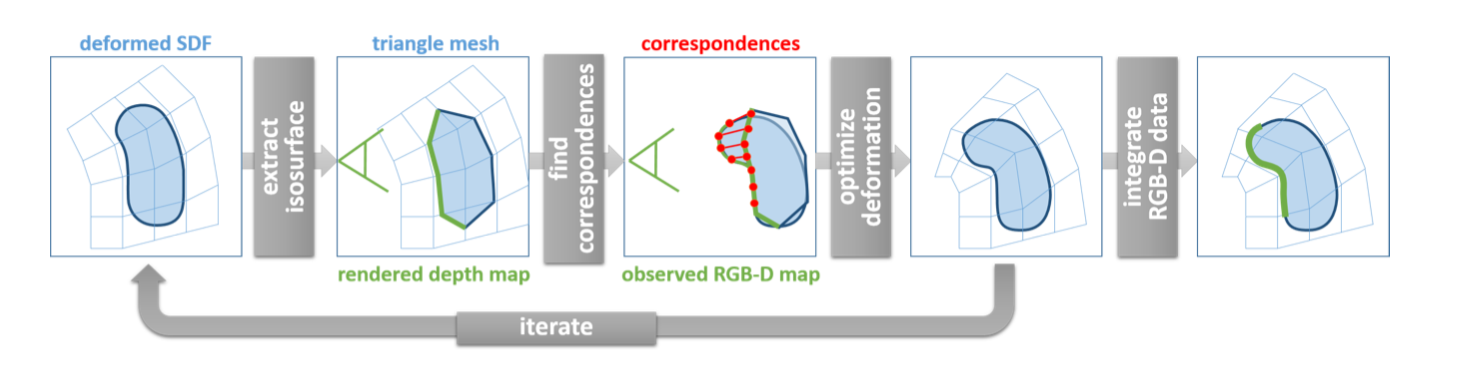
\includegraphics[width=12cm]{figures/pipeline.png}
\caption{Method Overview}
\label{fig:pipeline}
\end{figure}


\section{Implementation of TSDF}
\subsection{Data Structure}
TSDF(Truncated signed distance field) represents surface interfaces as zeros, free space as positive values that increase with distance from the nearest surface, and occupied space with a similarly negative value. Unlike SDF, it sacrifices a full signed distance field that extends indefinitely away from the surface geometry, but allows for local updates of the field based on partial observations. ~\cite{CanelhasDanielRicao2017Tsdf} Based on the depth map generated by Kinect, the field is truncated at a small negative and positive values, $D_{min}$ and $D_{max}$, respectively, produces the projective truncated signed distance field. For each voxel, it has a truncated distance $D{(x)}$, weighted by a measurement weight $W{(x)}$.

\begin{figure}[htp]
\centering
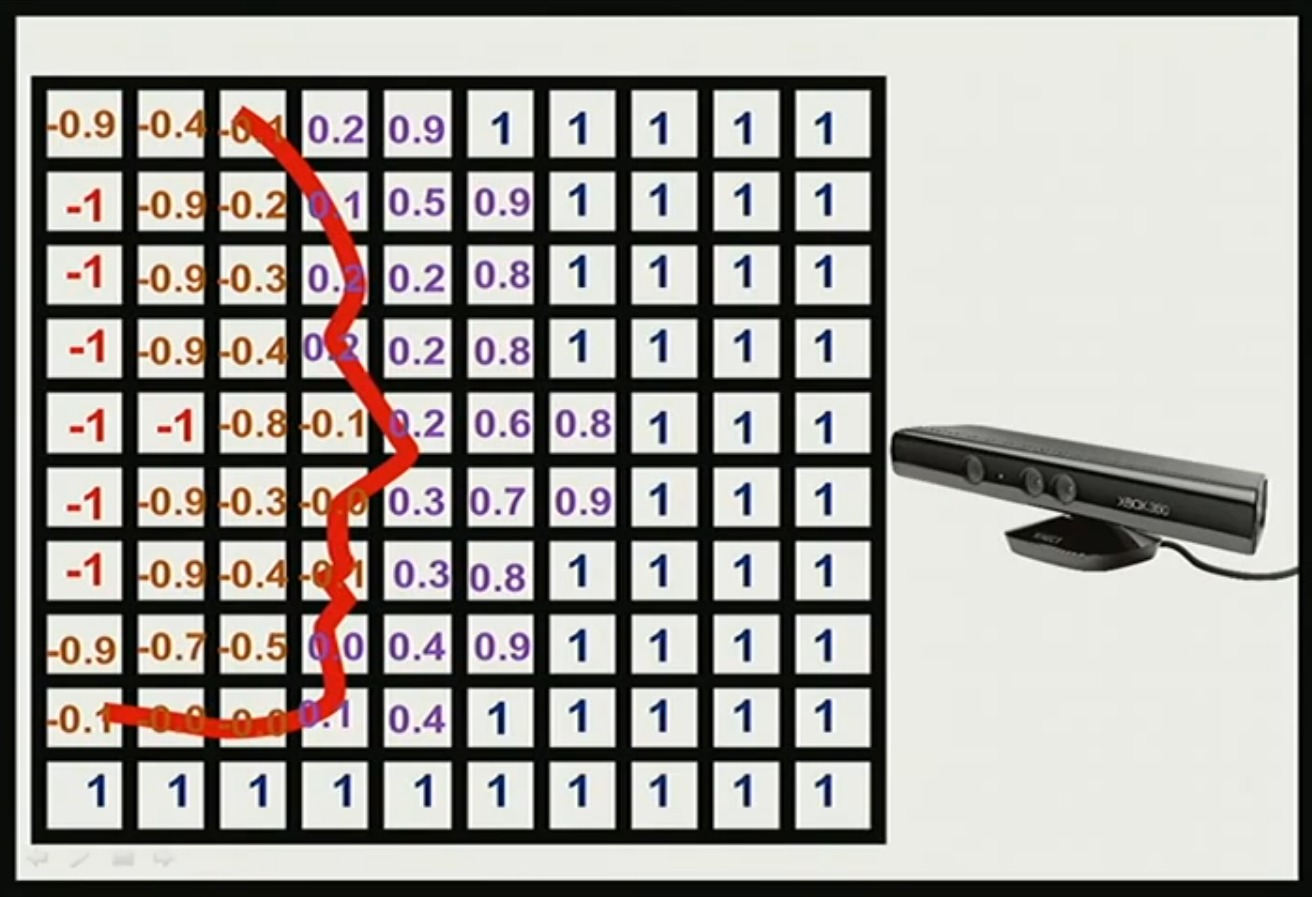
\includegraphics[width=6cm]{figures/tsdf.jpg}
\caption{The Structure of TSDF}
\label{fig:TSDF}
\end{figure}

Unlike the reconstruction of rigid objects in which all voxels are fixed in the world coordinate system, voxels may move while reconstructing non-rigid objects. Therefore, each voxel has its own coordinate and its 8 verteices also have coordinates, shown in Fig. 3(a). The voxel coordinates are calculated using trilinear interpolation algorithm with their surrounding 8 grid coordinates, shown in Fig. 3(b).

\begin{figure}
\centering
\begin{subfigure}{.65\textwidth}
  \centering
  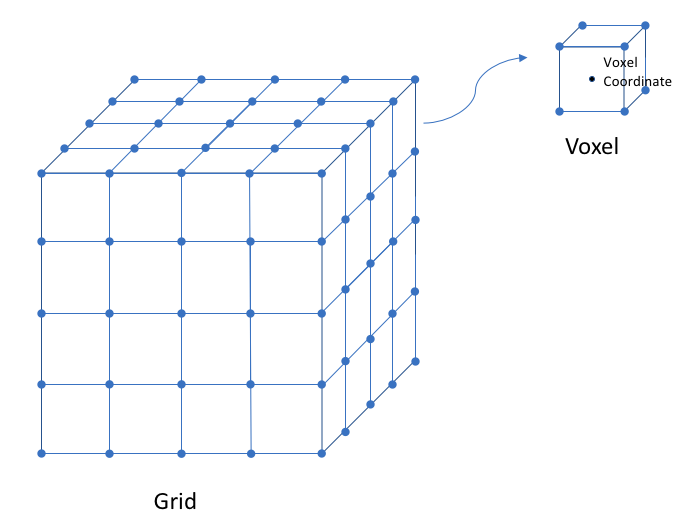
\includegraphics[width=.65\linewidth]{figures/DataStruct.png}
  \caption{TSDF Grid}
  \label{fig:sub1}
\end{subfigure}%
\begin{subfigure}{.35\textwidth}
  \centering
  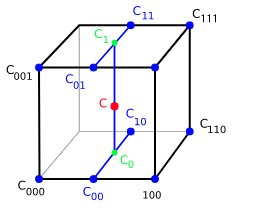
\includegraphics[width=.35\linewidth]{figures/3D_interpolation.png}
  \caption{Trilinear Interpolation}
  \label{fig:sub2}
\end{subfigure}
\caption{The Data Structure of TSDF}
\label{fig:test}
\end{figure}


\subsection{Initiation}
In order to draw the object in TSDF as accurate as possible, we assume that there is \(1m * 1m * 1m \) cubic space in the world coordinate and assume the size of each voxel is \(1mm * 1mm * 1mm \). Therefore, the dimension of TSDF in this project is \(1000 * 1000 * 1000\). As for the initiation of each voxel's distance and weight, we firstly cast them back to the depth frame, and then compare z value of the voxel and the depth value of corresponding pixel. The world-to-camera transformation matrices are provided by the dataset. In the end, the difference of these two values is truncated by a fixed value(In this project, the truncation margin is 0.5cm). For every voxel, their weights are initiated as 1.0.

\subsection{Integration}
Integration of a depth frame $D_i$ occurs as follows. For each voxel, $D{(x)}$ denotes the signed distance of the voxel,  $W{(x)}$ the voxel weight, $d_i{(x)}$ the projective distance (along the z axis) between a voxel and $D_i$, and $w_i{(x)}$ the integration weight for a sample of $D_i$. For data integration, each voxel is then updated by~\cite{dai2017bundlefusion}:

\[D'(x)=\frac{D(x)W(x)+d_i{(x)}w_i{(x)}}{W(x)+w_i{(x)}}\]

\[W'(x)=W(x)+w_i{(x)}\]
In this project, the integration weight $w_i{(x)}$ for a sample of $D_i$ is set as 1.0. We can thus update a frame in the reconstruction by integrating it with a new pose. This is crucial for obtaining high-quality reconstructions in the presence of loop closures and revisiting, since the already integrated surface measurements must be adapted to the continuously changing stream of pose estimates. Since the initialization and Integration are implemented in a parallel way, each voxel is allocated with a thread and the sudo code is shown below:

\begin{lstlisting}[language=C++]
For each voxel v:
    transform v from world coordinate into camera coordinate;
    // Using camera intrinsic matrix
    project v to get corresponding pixel p;
    
    diff = p.depth - v.z;

    if (diff <= -trunc_margin)
    	return;
    
    // Integrate
    dist = Min{1.0, diff / trunc_margin];
    W_new = W_old + 1.0f;
    D_new = (D_old * W_old + dist) / W_new;

    
\end{lstlisting}

\section{Implementation of Parallel Marching Cubes}

Marching cubes is a computer graphics algorithm came up by Lorensen and Cline~\cite{Lorensen:1987:MCH:37402.37422} for extracting a polygonal mesh of an isosurface from a logical cube created from eight voxels, four each from two adjacent slices,shown in Fig.~\ref{fig:tsdf_mc}. The algorithm determines how the surface intersects this cube, then moves (or marchs) to the next cube. To find the surface intersection in a cube, we have to know the positional relation between vertices of the cube and the surface, which have been known in TSDF. Cube vertices with $D{(x)}$ lower than zero are inside (or on) the surface and cube vertices with  $D{(x)}$ larger than zero are outside the surface. The surface intersects those cube edges where one vertex is outside the surface and the other is inside the surface. With this assumption, we determine the topology of the surface within a cube, finding the location of the intersection later. 

\begin{figure}[h]
\centering
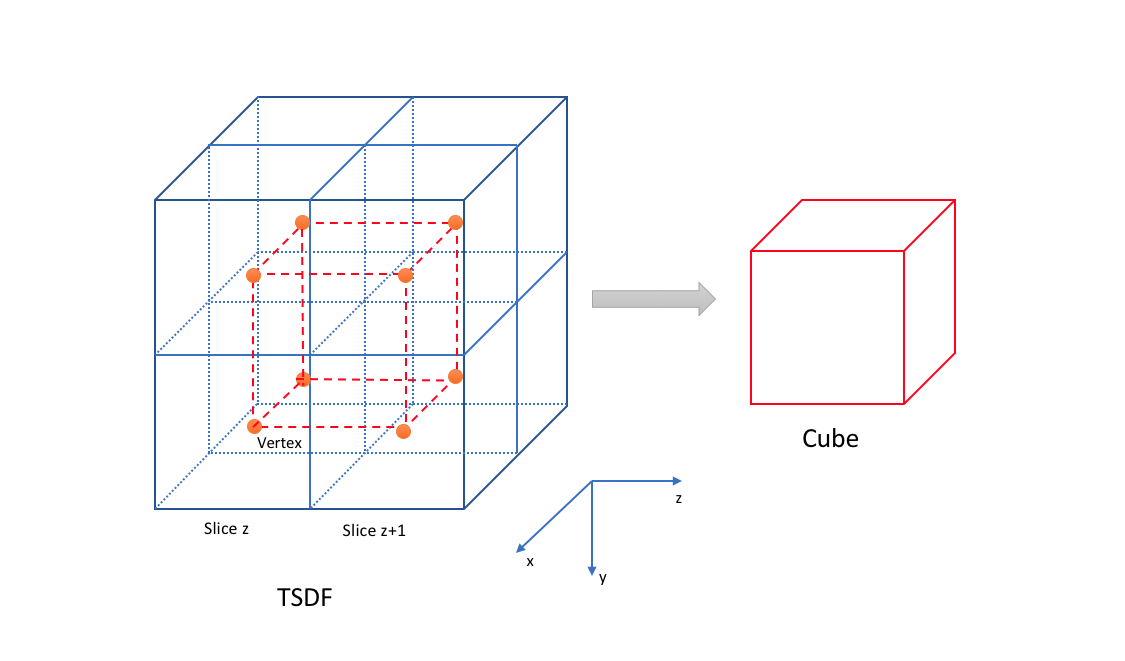
\includegraphics[width=9cm]{figures/TSDF_MC.png}
\caption{The cube in TSDF}
\label{fig:tsdf_mc}
\end{figure}

Since there are eight vertices in each cube and two slates, inside and outside, there are only $2^8 = 256$ ways a surface can intersect the cube. By enumerating these 256 cases, we create a table to look up surface-edge intersections, given the labeling of a cubes vertices. The table contains the edges intersected for each case. 256 cases can be summarized into 15 cases by eradicating symmetric cases, shown in Fig.~\ref{fig:triangulation}

\begin{figure}[h]
\centering
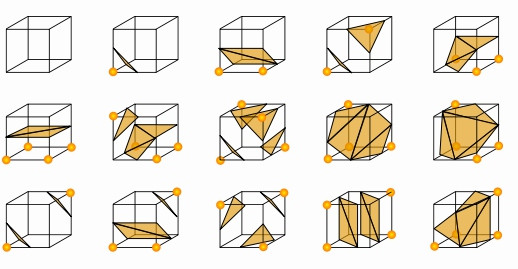
\includegraphics[width=9cm]{figures/mc.jpg}
\caption{Triangulated Cubes}
\label{fig:triangulation}
\end{figure}

We create an index for each case, based on the state of the vertex. Using the vertex numbering in Fig.~\ref{fig:cubenum}, the eight bit index contains one bit for each vertex. This index serves as a pointer into an edge table that gives all edge intersections for a given cube configuration. Using the index to tell which edge the surface intersects, we can interpolate the surface intersection along the edge. In general, we assume the intersection point is in the middle between two vertices. However, since each voxel has a weight, the coordinate of the intersection point is based on the difference between weights of two vertices as the following:

\[Ratio = ( 0 - W_{start} ) / ( W_{end} - W_{start})\]
\[\overrightarrow{Edge} = V_{end}- V_{start}\]
\[\overrightarrow{\triangle} = Ratio * \overrightarrow{Edge}\]
\[Intersection = V_{start} + \overrightarrow{\triangle}\]


\begin{figure}[h]
\centering
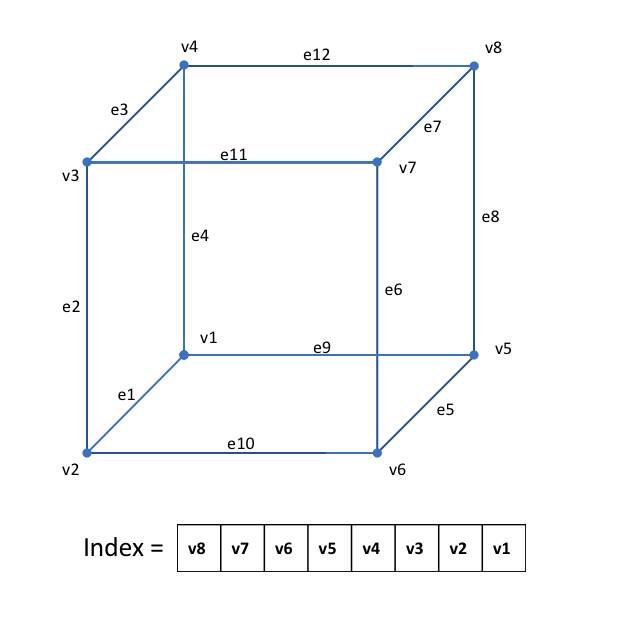
\includegraphics[width=6cm]{figures/Cubenum.png}
\caption{Cube Numbering}
\label{fig:cubenum}
\end{figure}

In this project, each voxel moves independently to reconstruct a non-rigid object. In other words, cubes used in this algorithm might not be regular cubes. However, we assume that the deformation of objects is tiny between two frames so the algorithm works well under this condition. 
\section{Result}
In order to focus on the reconstruction of main objects, we eliminate rigid background while reading depth frames. After initializing TSDF from the first frame, we apply marching cubes algorithm to it and then extract the mesh which is used as the input to the optimization of deformation. 
\begin{figure}[h]
\centering
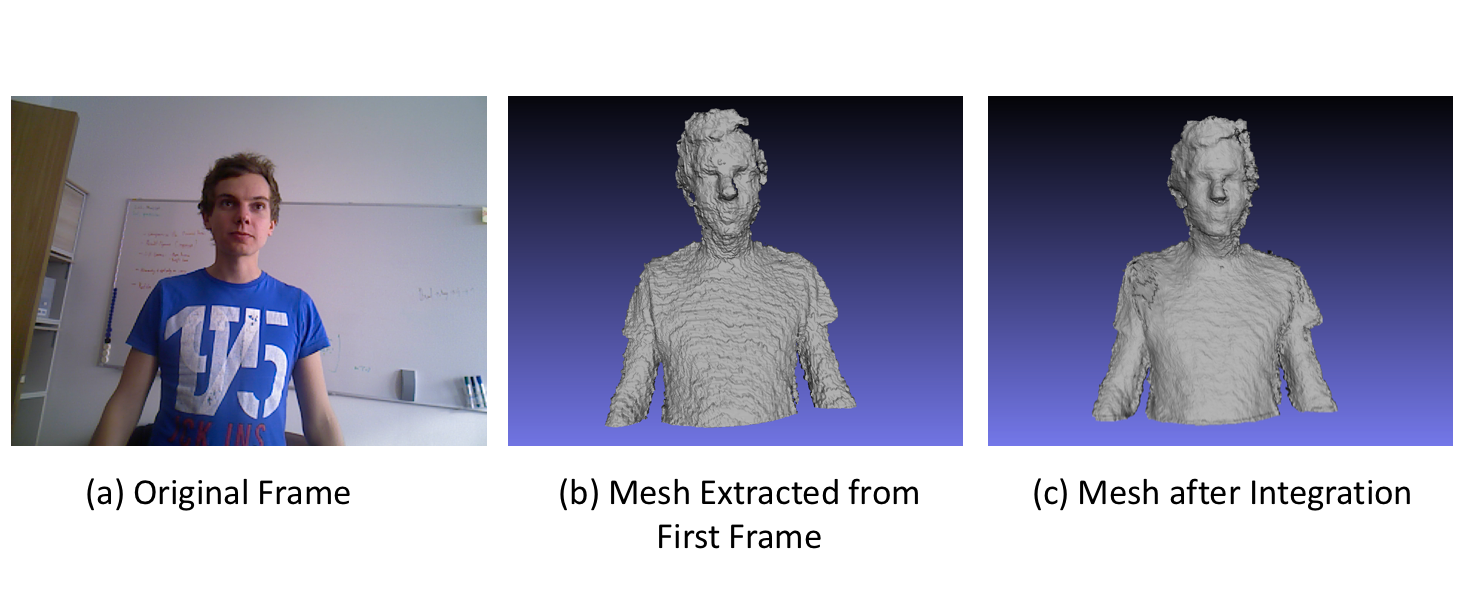
\includegraphics[width=10cm]{figures/upperbody.png}
\caption{ }
\label{fig:uppperbody}
\end{figure}
As Fig.~\ref{fig:uppperbody}(b) shows, the mesh extracted from the first frame is quite coarse and there are many noises. Fig.~\ref{fig:uppperbody}(c) shows the mesh after integrating 5 frames and we can see it becomes much smoother. However, noises still exist so we need to improve the robustness of marching cubes algorithms in the future.  

%\printbibliography
\bibliographystyle{unsrt}
\bibliography{references}

\end{document}
